%Vorlage
\documentclass[12pt,a4paper]{scrartcl}
\usepackage[english]{babel} %Für die indirekte Angabe von Umlauten. Es müssen dann Umlaute wie folgt im Code angegeben werden: "a "o "u "s.

\usepackage[utf8]{inputenc}
%Math
\usepackage{amsmath, amsthm, amssymb}
\usepackage{braket}
\newcommand{\tens}[1]{% https://tex.stackexchange.com/questions/171788/always-have-the-ring-of-the-tensor-product-below-the-otimes -> Tensor Product
  \mathbin{\mathop{\otimes}\displaylimits_{#1}}%
}
%Page numbers
\usepackage{enumerate}
%Graphics
\usepackage{graphicx}
\usepackage{array}% http://ctan.org/pkg/array
\usepackage{floatrow}
\graphicspath{{./images/}}
%Quantum circuits http://mirrors.ibiblio.org/CTAN/graphics/pgf/contrib/quantikz/quantikz.pdf
\usepackage{tikz}
\usetikzlibrary{quantikz}
\usepackage{lscape}
\usepackage{setspace}
\onehalfspacing
\usepackage{wrapfig}
\usepackage{hyperref}% für die Einbettung von Hyperlinks
\def\UrlBreaks{\do\/\do-}
\usepackage{multirow}
\usepackage{csquotes} %Quotations
%Code
\usepackage{pythonhighlight}


% Margins
%\usepackage{geometry} % Document Margins
%\setlength{\topmargin}{0cm}
%\setlength{\parindent}{5mm}
%\setlength{\parskip}{2mm}
%\setlength{\evensidemargin}{0mm}
%\setlength{\oddsidemargin}{0cm}
\pagestyle{headings}



\begin{document}
\thispagestyle{empty}
\vspace*{-3cm}
\begin{center}
\large \textsc{Bern University of Applied Sciences}
\vspace{0.5cm}
\hrule
\vspace{3.5cm}
{\Large \textsc{Written Report\\
Bachelor Thesis}}\\
{\large HS 2020/21}\\
\vspace{1cm}
{\Large \bfseries
Generation of synthetic ground truth for ophthalmic medical image analysis}\\

\vspace*{1cm}
{\large Tutor:  Prof. Dr. Tiziano Ronchetti}
\end{center}
\vspace*{1cm}

\begin{abstract}
As machine learning becomes ubiquitous in the software engineering world, more and more projects are dedicated to implement the technology in the life sciences field. In this report we propose a framework that process ophthalmic OCT images and predicts synthetic vitreal, retinal, choroidal and scleral semantic segmentations based on a combination of image augmentation techniques and a convolutional neural network presenting an encoder-decoder structure. After cross-validation the results indicate that our framework can automatically segment a regular OCT scan with a mean Jaccard coefficient of 96,87\%, showcasing a Hamming distance of xx\% when compared to human ophthalmologists. In addition, we present a detailed workflow involving the utilisation of state-of-the-art machine learning techniques with comprehensive explanations on the data preparation, model implementation and evaluation criteria.  
\end{abstract}

\vspace{2cm}
\hspace*{5.2cm}
\parbox{8.2cm}

\begin{tabular}{ll}

Submitted by: & Emeline Liebeherr\\
& Rayner Zorrilla Alfonzo\\

Submission deadline: & Thursday, June 17th, 2021


\end{tabular}

\newpage
\pagenumbering{Roman}
\tableofcontents

\newpage
\pagenumbering{arabic}
%Und nun kommen wir zur Arbeit und fangen an die Seiten mit Arabischen Zahlen zu zählen

\section{Introduction}\label{s:introduction} 
\subsection{Motivation}\label{ss:motivation}
The choroid is the vascular layer of the eye. It contains connective tissues and is located between the sclera on the outside and the retina on the inside. The choroid is responsible for the irrigation and circulation of the ocular metabolism in order to supply the outer retina with oxygen and metabolites\cite{choroidExpl}.

Its thickness can depend on several factors, including age, blood pressure, anatomic pathologies, etc. It has been found that the thickness of the choroid decreases with age, however several recent research studies on choroidal development during childhood and adolescence contradict this finding. In particular, subfoveal choroidal thickness has been found to be negatively correlated in Asian children, where the prevalence of myopia is higher\cite{Ronchetti2019}. Longitudinal studies of adolescents have shown that the eyeball lengthens during the development of myopia \cite{Ronchetti2018}. In the case of severe myopia this process is associated with a significant thinning of the choroidal thickness. Therefore the choroidal structure and thickness are strongly considered for monitoring the progression of myopia\cite{Ronchetti2019}.

The main challenge in detecting disease progression is to detect even small changes as early as possible. Optical coherence tomography (OCT) imaging allows the capture of highly resolved details of the retina and choroid to detect minute changes in the structure of both membranes\cite{Ronchetti2019}.

In order to measure these changes in choroidal thickness it is necessary to detect all the different layers present in the ocular globe's peripheria and their interfaces from OCT scans. With such segmentation one can compare results over several years. 
However, a manual approach raises two important problems: firstly, the number of scans to be processed (layer identification) is considerable \cite{Maloca2019}. Secondly, the low contrast, loss of signal, and the presence of other image degradations mentioned in Sec.\ref{ss:motivation} the choroid makes it difficult to distinguish the sclera from that of the choroidal border \cite{Ronchetti2019}.

\subsection{Goal}
The aim of this project is to develop a deep learning model able to process  ophthalmic  OCT  images  and to predict  synthetic  vitreal,  retinal,  choroidal  and  scleral  semantic  segmentations  based  on  a  combination  of  image  augmentation  techniques  and  a convolutional neural network presenting an encoder-decoder structure with a mean Jaccard coefficient of at least 95\%   \cite{Maloca2019}. This will automate the measurements made on the scans and considerably reduce the time needed to produce a result, thus reducing the workload of the experts and ensuring a certain accuracy and standardization in the detection of the choroid. 

\subsection{Contributions}

The contribution of this project lies in the setup and documentation of a software framework capable of generating ground truth images for ophthalmic image medical analysis where the vitreal, retinal, choroidal and scleral compartments are clearly defined. The mentioned framework includes image pre-processing, model implementation and results evaluation. 

From a medical perspective, the final output offers health care providers and other experts an image where the major layers present in a regular OCT scan are pre-segmented with a high degree of confidence, which can form the basis of different analysis involving choroidal and retinal thickness. 

\subsection{Material and Methods}

\subsubsection{Methodology}

A Convolutional Neural Network (CNN) was designed based on the U-Net CNN model created by Prof.~Dr.~O.~Ronneberger in 2015 \cite{Ronneberger2015}. According to the general machine learning worklow, we used different techniques of data pre-processing that include vectorization, categorization and augmentation of the annotated images in order to train the network. Hyperparameters were modified both empirically from the result of several training sessions and by using best algorithmic practices for weighting and learning rate selection. Finally, the images resulting of the CNN predictions are evaluated by using different metrics commonly tracked on machine learning projects like the Dice and Jaccard coefficients, sensitivity, specificity and for evaluating the loss a weighted version of the categorical crossentropy. 

\subsubsection{Data}

For this project we used a dataset composed of 755 OCT B-scans\footnote{See Sec. \ref{s:TechBack} for more information.} of 500*768 pixels. The data was obtained from asian patients in the age range of 8-18 years stemming from urban regions with a high prevalence of myopia. The subject were healthy with globally good distance and near vision, no systemic and ocular diseases, ocular trauma or surgery\cite{Ronchetti2019}. The images were acquired by a dual-wavelength eye-tracking OCT system operating simultaneously at the 870 and 1075 nm bands. This system was developed by HuCE-opto-Lab at the Bern University of Applied Sciences in Biel, Switzerland \cite{Ronchetti2019} \footnote{For more information about the OCT dataset we refer the interest reader to \cite{Ronchetti2019}}.

\subsubsection{Tools}
The framework at its current state is dependent on the following tools : 
    
    \begin{table}[H]
    \begin{tabular}{ll}
    Tool & Version \\
    Python & 3.8.5 \\
    Keras     & 2.4.3   \\
    Tensorflow & 2.4.0 \\
    Opencv-python  &   4.5.1.48 \\
    Numpy & 1.19.2 \\
    Glob2  &  0.7 \\
    Matplotlib & 3.3.2
    \end{tabular}
    \end{table}



\section{Medical Background}\label{s:medical_background}

The human eye is a sensory organ that is composed by two different segments of spheres named the anterior and posterior segments \cite{snell1998}.

The anterior segment is the most front part of the eye, it hosts the cornea, iris and lens and serves to regulate the intensity of the light that is transmitted to the retina which is located in the posterior segment of the eye alongside the vitreous body, choroid and sclera. The function of the posterior segment is to convert light waves into electrical signals that are interpreted by the brain in the form of images \cite{Rhoades2017}. 

\begin{figure}[H]
    \centering
    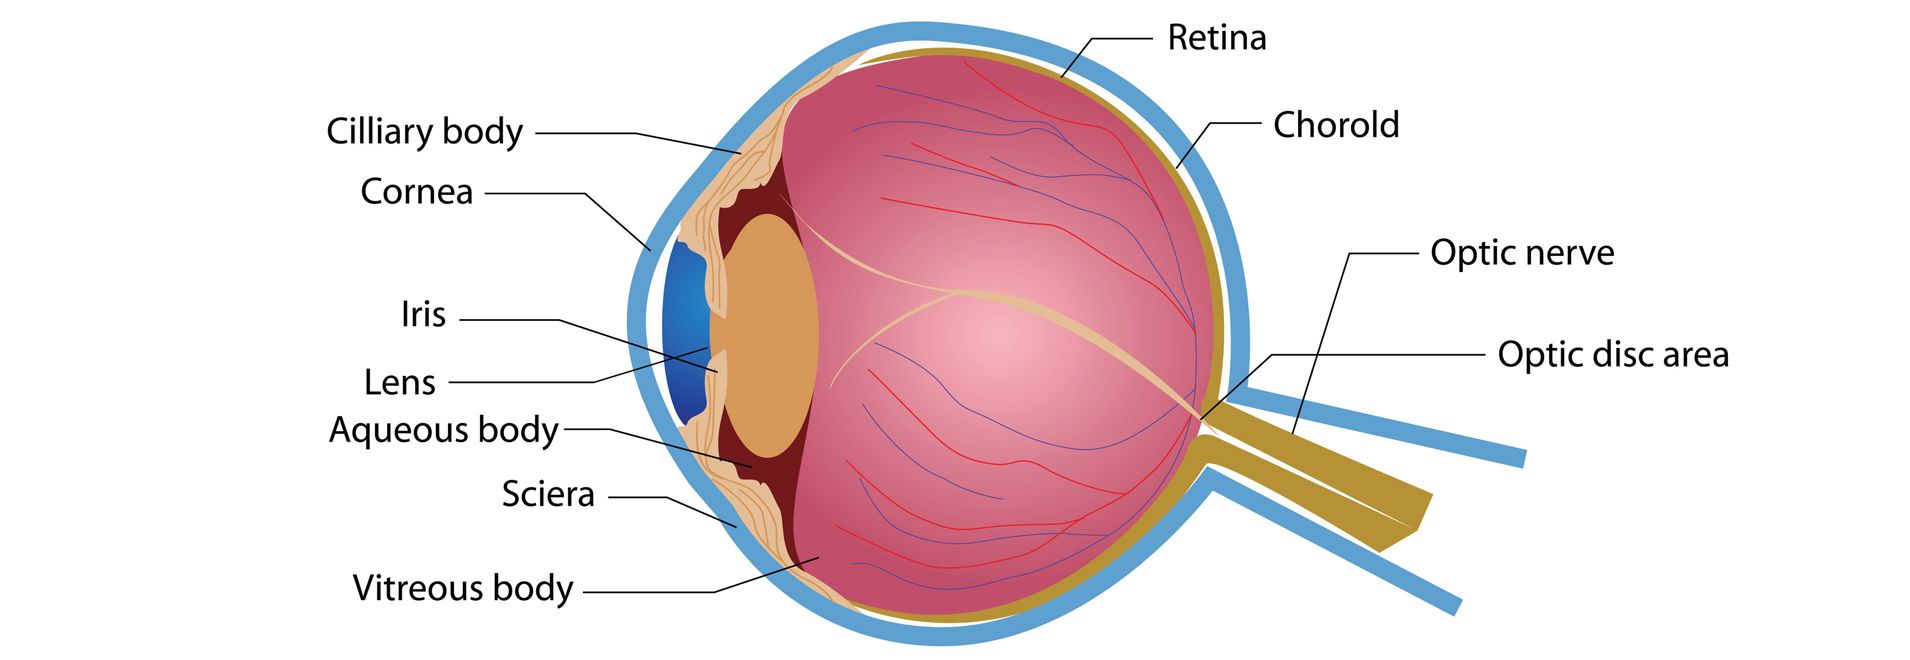
\includegraphics[width=0.8\textwidth]{./images/anatomy-of-the-eye.jpg}
    \caption{Anatomy of the eye \cite{eyeanatomy-pic}}
    \label{fig:eye-anatomy}
\end{figure}

The area of interest of this report is limited to the posterior segment of the eyeball as the tissues that are present in it have significant clinical value to ophthalmologists in the analysis and diagnosis of refractive errors (myopia) and other other ocular diseases (glaucoma)\cite{Ronchetti2017}. In particular, we will focus in the vitreous body, retina, choroid and sclera as they will form integral part of the set of annotations developed for our research in the field of machine learning. 

The vitreous body is an structure characterized by a colorless and transparent gel. It's mainly composed by water and other aminoacids, proteins, salts and acids. The vitreous located between the lens and the retina and occupies 4/5 of the total volume of the eye and serves mainly to transmit light from the lens to the retina. It's also believed that it contributes to the convergence power of the eye \cite{snell1998}. 

Once the light has traveled through the vitreous body, it reaches the retina which is a tissue layer envolving the vitreous. As a part of the central nervous system, the retina transforms light waves captured its photoreceptors into electric signals that travel to the brain via the optic nerve \cite{purves2001}. In other terms, it converts light into electric signals that are sent to the brain and are interpreted as images.

Supporting the retinal function, between the retina and sclera, the choroid irrigates the outer retina with oxigen due to it's vascular structure through an intrincated layer of capillaries which are connected to arteries via the choroid's vessel layer \cite{snell1998, choroidExpl}. Several studies \cite{Ronchetti2019, Ronchetti2018} indicate that choroidal thickness has a positive correlation with the development of myopia, which is part of the motivation of this work. 

Finally, the sclera protects the inner part of the ocular globe due to its collagenous structure. Together with the cornea, it serves to contain the internal pressure of the eye and also to contain the forces created by the external muscles of the eye during eye movement \cite{Meek2008}.

\section{Technical Background}\label{s:TechBack}


\subsection{Optical Coherence Tomography}
Optical Coherence Tomography (OCT) is the standard technique for producing accurate visualizations of ophthalmic medical images \cite{Garrido2014}. Since OCT uses near-infrared low-coherence light waves to produce measurements of the reflectivity vs. depth (also known as A-scans\cite{Garrido2014}) it represents a non-invasive procedure to extract information from the ocular globe structure. Several A-scans from consecutive zones can be combined in order to form a 2D image of the posterior segment of the eye where the vitreous, retina, choroid and sclera can be clearly located. Finally, a contiguous set of B-scans produces a volumetric image that ophtalmologist can use to first evaluate the retinal and choroidal structure and second calculate the layers thickness and issue diagnoses on several type of diseases including various ocular diseases \cite{Ronchetti2019}, Diabetes \cite{Jiang2018}, Alzheimer, Glaucoma and other neurodegenerative diseases \cite{DENHAAN2017162}.   


\begin{figure}[H]
    \centering
    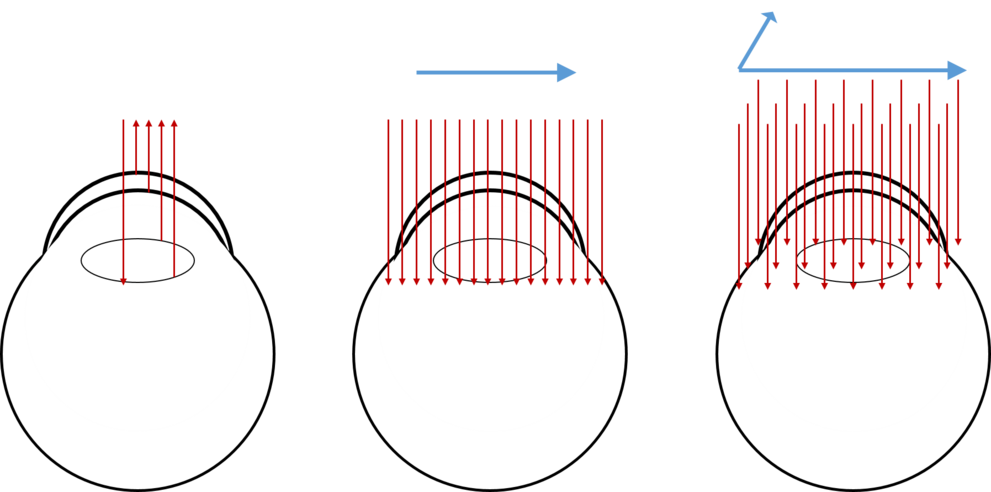
\includegraphics[width=0.8\textwidth]{./images/csm_ABC_scans.png}
    \caption{Scan Types in Optical Coherence Tomography \cite{Willdeman2016}. From left to right: A-scan use a signal depth profile composed of time-gates reflections; B-scan use a frame composed of array of A-scans; Volume use a 3D Dataset composed of array of B-scans.}
    \label{fig:mb-oct-abcscans}
\end{figure}

As stated in the motivation of this thesis, retinal and choroidal thickness can be measured from OCT scans with the help of annotated ground truths establishing the locations of the tissues' boundaries. In the case of the retina, the Internal Limiting Membrane (ILM) divides it from Vitreous on the upper boundary \cite{MACNAIR2015343}, while the Bruchs Membrane (BM) divides the retina from the choroid \cite{BOOIJ20101} serving as the retina's bottom boundary. Subsequently, the Choroidal-Scleral Interface separates the choroid from the sclera \cite{Ronchetti2018}. The mentioned boundaries create a segmentation map within OCT B-Scans where the vitreous body, retina, choroid and sclera can be analysed as presented in Fig.~\ref{fig:annotated-oct-scan}. 


\begin{figure}[H]
    \centering
    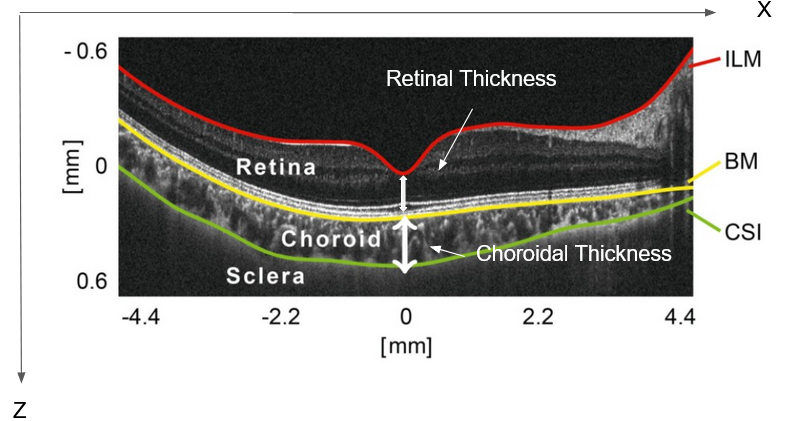
\includegraphics[width=0.8\textwidth]{./images/OCT-Scan.png}
    \caption{A B-scan with segmented layers from top to bottom:  Internal Limiting Membrane (ILM),  Bruch's Membrane (BM), Choroid-Sclera Interface (CSI) \cite{Ronchetti2019}}
    \label{fig:annotated-oct-scan}
\end{figure}

\subsection{Convolutional Neural Networks}\label{s:cnn}

A CNN is a powerful family of neural networks inspired by biological processes and containing Convolutional Layers, used in the field of deep learning. The design of the connection pattern is inspired from the structure of the neurons in the visual cortex of animals. Modern CNNs are effective in obtaining accurate models, as they require fewer parameters than fully connected architectures, and are often more computationally efficient because convolutions are easily parallelized on GPU cores\cite{DIDLBook}. Furthermore, CNN-based architectures are common in the computer vision field, as they are prized for their efficiency. 

To be functional, Convolutional Networks need some operations, the techniques used by CNN to capture features from images is achieved by applying a series of operations known as convolutions and pooling, both of them will be described in this chapter. 

In the case where one wishes to process datasets by collecting and annotating pixels of images one can quickly end up with a network having huge dimensions leading to poor GPU performance, for this reason CNNs are used for data that is not tabular\footnote{by tabular we mean data consisting of rows corresponding to examples and columns corresponding to features}\cite{DIDLBook}. The main role of the CNN is to facilitate the processing of images by reducing them to a form that is easier to examine without losing the features that are essential in the obtaining of a good prediction.

\subsubsection{Convolution Operation}
An important concept of CNN is spatial invariance, which means that object recognition is not sensitive to their position in the image. In computer vision, adding convolution to the neural network allows the addition of an inductive visual prior whereby objects can appear anywhere.  Sharing the weights over the location of the object significantly reduces the parameters to be learned, the convolution is moved when the object change position \cite{CNNSpatialLocation}. The earliest layers of our network should be implementing translation invariance, meaning that it should respond similarly  regardless of where the objects appears in the image. And they should focus on local regions (locality principle) without regard for the contents of the image in distant regions. \cite{DIDLBook}

The translation invariance implies that a shift in the input \(x\) should lead to a shift in the hidden representation \(H\) (represented as matrices in mathematics and as two-dimensional tensors in code). 
This is a convolution as the weighting pixels at \((i + a, j + b)\) in the vicinity of location
\((i, j)\) with coefficients \([V]_{a,b}\) to obtain the value \([H]_{i,j}\) .: 
\begin{equation}
\label{eqn:invariance}
[H]_{i,j} = u + \sum_a\sum_b[V]_{a,b}[X]_{i+a,j+b}
\end{equation}
Note that both X and H have the same shape and \([X]_{i,j}\) and \([H]_{i,j}\) denote the pixel at location \((i, j)\) in the input image and hidden representation. The translation invariance is only possible if V and u do not depend on \((i, j)\) \cite{DIDLBook}.
As described above, in the locality principle , it should no not be necessary to look far away from the location \((i, j)\) to retrives informations to describe what happens in \([H]_{i,j}\), outside a certain range \(|a| > \Delta \) or \(|b| > \Delta\), we should set  \([V]_{a,b} = 0\). And rewrite \([H]_{i,j}\) as follow \cite{DIDLBook}:
\begin{equation}
\label{eqn:locality}
[H]_{i,j} = u + \sum_{a=-\Delta}^{\Delta}\sum_{b=-\Delta}^{\Delta}[V]_{a,b}[X]_{i+a,j+b}
\end{equation}

The operation for the spatial invariance \ref{eqn:invariance} and the locality \ref{eqn:locality} are convolutions since in mathematics the convolution between two function \(f\) and \(g\) with \({\rm I\!R}^d \rightarrow {\rm I\!R}\) is defined as follow \cite{DIDLBook}: 
\begin{equation}
(f*g)(x) = \int f(z)g(x-z)dz
\end{equation}
(The function measures the overlap between \(f\) and \(g\) when one of the functions is “flipped” and shifted by \(x\). If we use two-dimensional tensors, we have a corresponding sum with indices \((a b)\) for \(f\) and \((i-a, j-b)\) for \(g\), that is very similar to \ref{eqn:locality} (exception of the use of \((i+a, j+b)\) instead) \cite{DIDLBook}:
\begin{equation}
(f*g)(i,j) = \sum_{a}\sum_{b} f(a,b)g(i-a,j-b)
\end{equation}

\subsubsection{Pooling Operation}
In general, when the need to process images arises, the most efficient way is to progressively reduce the detail of an image (for a given dimension) of our hidden representations. Thus, the higher one goes in the network, the larger the field of perception becomes, so the more the perceived image is composed of generalities and not of details. The final task we want to perform is generally a global one, in the case of this work: to find out where the borderlines between the ILM, the BM and the CSI is. This is why the layers of our network should be sensitive to all the inputs in order to have a global view, this can be achieved by progressively accepting data and producing coarser maps but keeping all the advantages of convolutional layers at the intermediate processing layers. Just as when we want to detect edges, our representation must be invariant to translation as the change of even one pixel can significantly change the image. This is why pooling layers are used, which have the dual purpose of mitigating the location sensitivity of convolutional layers and spatially downsampling the representations. There are several types of (deterministic) pooling operations, here we will discuss max-pooling and average-pooling \cite{DFTPooling}. Like convolutional layers, pooling operators operate on a window of fixed size that moves through the different regions according to their stride \cite{DIDLBook}.
An example found in \cite{DIDLBook} shows how these operators work. If we take a 3x3 matrix representing our input, and imagine that the operator moves from left to right and up and down from the top-left corner, a max pooling operation will produce a new 2x2 matrix: 

\begin{figure}[H]
    \centering
    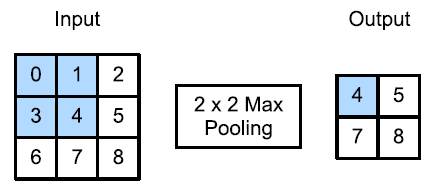
\includegraphics[width=0.8\textwidth]{./images/pooling_example.png}
    \caption{Pooling Operation example  \cite{DIDLBook}}
\end{figure}
Basically the max-pooling operation is to take the max value of a part of matrix (left blue) and place it in a new matrix (right) and then move and repeat this possess until the new matrix is populated.
\[max(0, 1, 3, 4) = 4,\]
\[max(1, 2, 4, 5) = 5,\]
\[max(3, 4, 6, 7) = 7,\]
\[max(4, 5, 7, 8) = 8.\]


as well as average -pooling would have given:
\[average (0, 1, 3, 4) = 2,\]
\[average (1, 2, 4, 5) = 3,\]
\[average (3, 4, 6, 7) = 5,\]
\[average (4, 5, 7, 8) = 6.\]

\subsubsection{Softmax Operation}
The Softmax function is a logistic function generalized to multiple dimensions and is used as an activation function for Neural Network. It is used to normalize the input vector z of K real numbers to a distribution consisting of K probabilities over predicted output classes. In this project we have four classes (vitreous, retina, choroid, sclera), therefore using softmax is relevant since it is a classifier which has excellent performance for multi-classification tasks and will often be used as the final layer of the network \cite{SoftMaxClassification}. 
The traditional softmax classifier can be described as follow: let  K be the number of classes, \(z_i\) we obtain  label and \(z_j\) the j-the element of the vector of class scores \cite{SoftMaxClassification, DIDLBook} :

\begin{equation}
\sigma(z_{ij}) = \frac{\exp{z_i}}{\sum_{j=1}^{K} \exp{z_j}}
\end{equation}
Once the convolution and pooling function have repeated until we have a pixel to be classified, the softmax function is used to determine the probability that this pixel belong to a certain class.

\subsection{U-net}

U-net is a CNN architecture developed for the field of biological images where samples are scarce and the outputs involve assigning certain regions of the image to one or more classes. Previously, an sliding window was the standard method to perform this task, but the method is computationally expensive and requires an enormous amount of time depending on the image dimensions \cite{Ronneberger2015}. Therefore, in 2015 Prof. Dr. Olaf Ronneberger from the University of Freiburg in Germany developed an architecture consisting first of a contracting or encoding path that uses a combination of convolutional and pooling operations in order to aggregate and classify pixels. Once the pixel has been recognized the architecture proposes a second expansive path using up-sampling operations where the classified pixels are concatenated with features from the contracting or decoding path to add localization information. 

\begin{figure}[H]
    \centering
    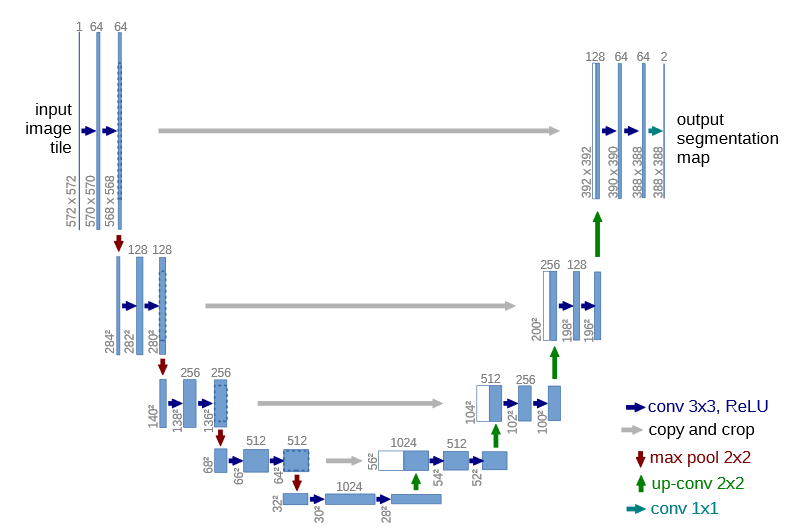
\includegraphics[width=0.8\textwidth]{./images/Unet-architecture.png}
    \caption{U-net architecture \cite{Ronneberger2015}. The blue boxes represent multichannel feature maps while the arrows represent the different mathematical operations described in Sec. \ref{s:cnn}    }
\end{figure}

The architecture is faster and less expensive than sliding windows since pixel features are aggregated to avoid classifying them individually. The second most important contribution of the paper is the idea of using image augmentation to circumvent the problem of image scarcity. By augmenting the image dataset, we apply a series of common image transformation operations in order to slightly modify the base image and create synthetic copies that reinforce learning. The detail of these operations is explained in Sec. \ref{ss:datapreparation}.

\section{Previous Work}\label{s:prevWork}
\subsection{Computer vision methods for detection of early choroidal thickness changes in myopic Asian school children}
\subsection{Literature Review}
There has been efforts to automate OCT scan segmentation using deep learning methods, although one of its principal limitations is described in Ronchetti et al. \cite{Ronchetti2019} and Alonso-Caneiro et al. \cite{Alonso-Caneiro2013} as a low degree of interannotator agreement when detecting the CSI, which would introduce significant differences in the class segmentation and consequently would lead to inconsistencies in choroidal and retinal thickness measurements. Moreover, it has been shown in \cite{Maloca2021} that the performance of deep learning methods is at it's best an average of the experts' annotations.

In 2017, Roy et al. \cite{Roy2017} proposed a fully convolutional deep learning architecture to segment retinal layers and fluid masses in OCT scans called ReLayNet. The architecture is used to train a joint loss function composed by  a weighted logistic regression and a Dice overlap. It proposes a similar encoder-decoder architecture using convolutional and pooling operations and additionally adding a softmax operation block for classifying pixels.

\begin{figure}[H]
    \centering
    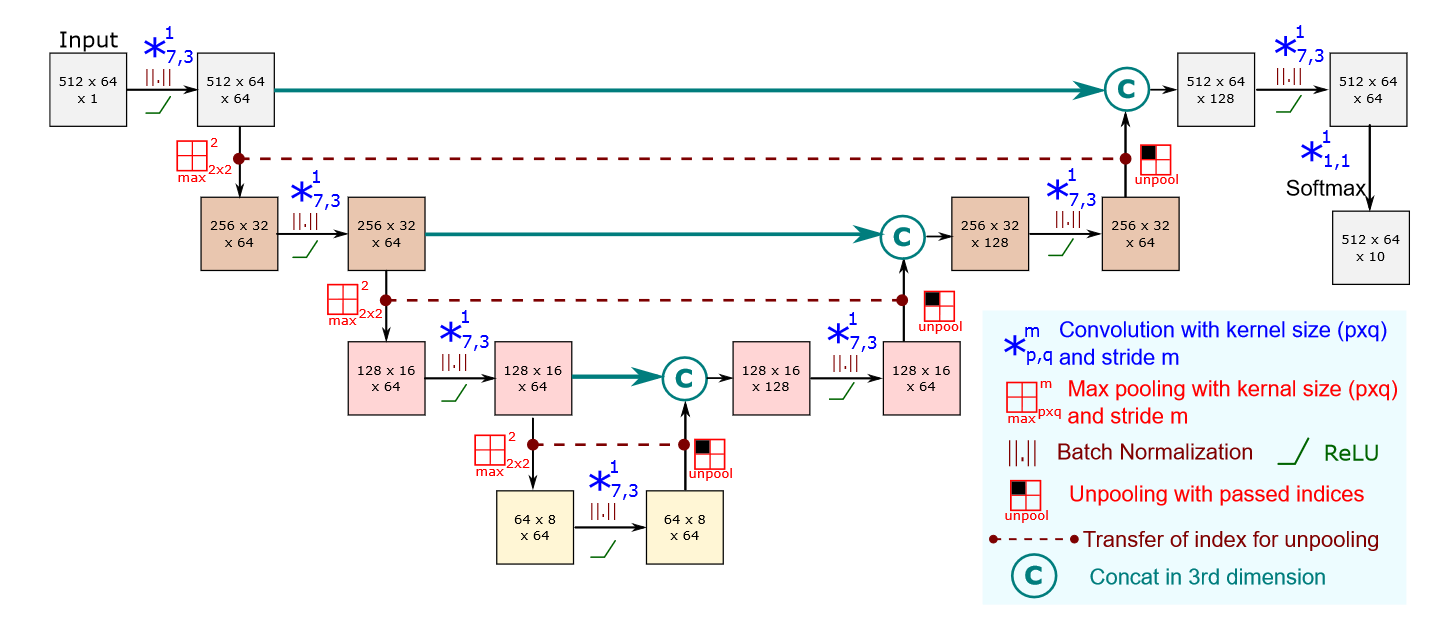
\includegraphics[width=0.8\textwidth]{./images/relaynet-architecture.png}
    \caption{ReLaynet architecture \cite{Roy2017}.}
\end{figure}

The model was trained in a dataset composed by 110 OCT B-scans of size 512*740 pixels annotated by two expert ophtalmologists. Using a 8-fold cross validation method, the results indicate a higher dice overlap score against other common used methods as U-net or FCN.

\begin{figure}[H]
    \centering
    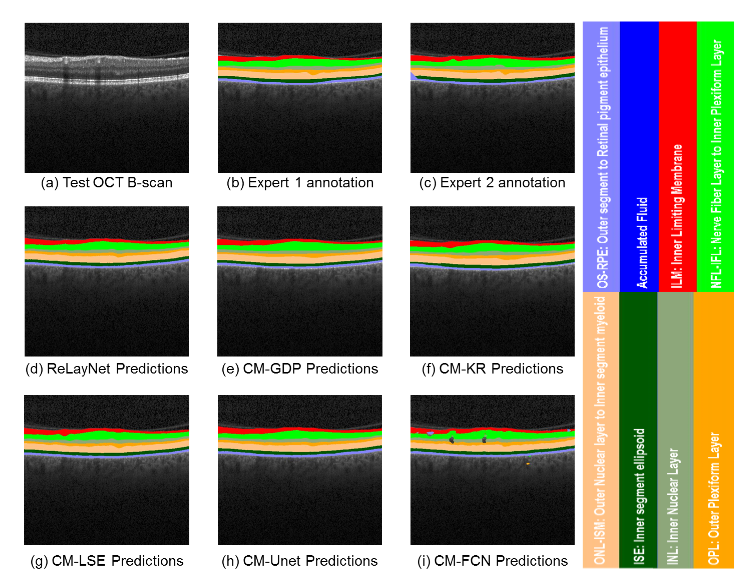
\includegraphics[width=0.8\textwidth]{./images/relaynet-predictions.png}
    \caption{OCT B-scan predictions using ReLaynet architecture model. In average the proposed model had a ILM's dice overlap score of 0.90 against U-net's 0.86 and 0,87 for the model known as Layer specific structured edge learning with  Graph based dynamic programming  \cite{Roy2017}.}
\end{figure}

Maloca et al. \cite{Maloca2019} validated the usage of deep learning methods by implementing a U-net CNN trained on a dataset of 2070 B-scans. The data was annotated manually by segmenting 4 compartments corresponding to the vitreous, retina, choroid and sclera. This was performed by identifying the ILM, the choriocapillaris (CC) and CSI. In this work the use of the choriocapillaris was preferred due to the thinness of the BM in OCT scans which makes it unrecognizable.

\begin{figure}[H]
    \centering
    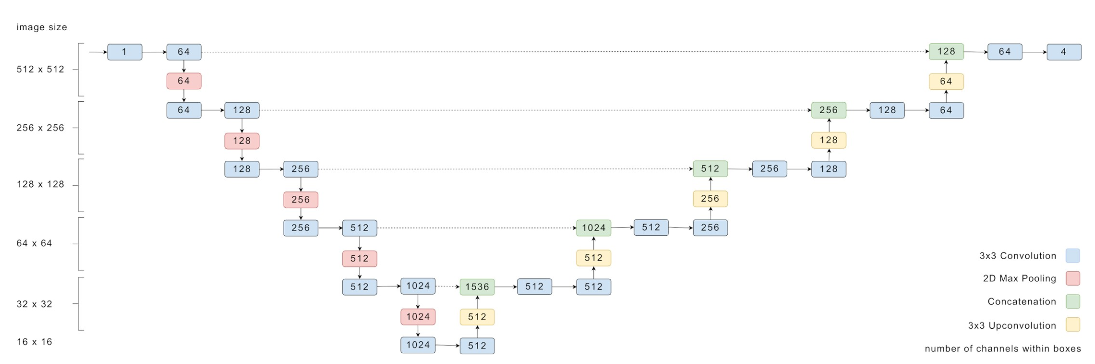
\includegraphics[width=0.8\textwidth]{./images/maloca-unet.png}
    \caption{Description of the U-net model used in \cite{Maloca2019}}
\end{figure}

The metric used to measure the performance of the U-net model in \cite{Maloca2019} was the Intersection over Union (IoC) also known as Jaccard coefficient, where all the matching pixels between both images are divided between the total of pixels of both images, giving a clear measure of similarity between both images. The results indicate mean IoU scores of 0.9929 for vitreous, 0.9690 for retina, 0.8819 for choroid and 0.9768 for sclera when benchmarked to a validation dataset of 60 images. From these results the authors concluded that the outputs of the proposed CNN were on par with manual segmentations made by human experts.

\begin{figure}[H]
    \centering
    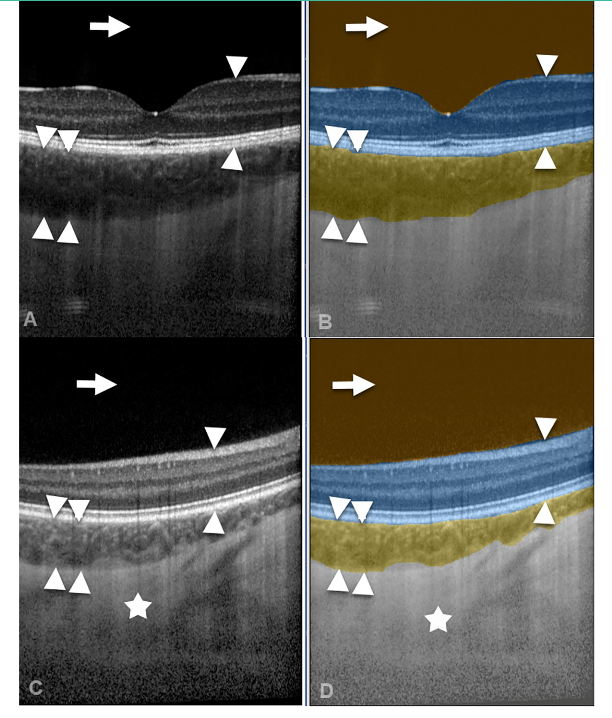
\includegraphics[width=0.7\textwidth]{./images/maloca-segmentations-results.png}
    \caption{Illustration of the predictions made by Maloca et al. A spectral-domain OCT image (A) and a swept-source OCT image (C) were automatically segmented by the CNN (B,D) in to the compartments vitreous (arrow), retina (arrowheads), choroid (double arrow heads), and sclera (asterisk) \cite{Maloca2019}.}
\end{figure}


Zheng et al. \cite{Zheng2020} proposed using a modified U-net architecture for automated segmentation of the choroid based on the Residual U-net model (ResNet) \cite{He2015} achieving higher performance with fewer parameters by using layers of residual functions. 
\begin{figure}[H]
    \centering
    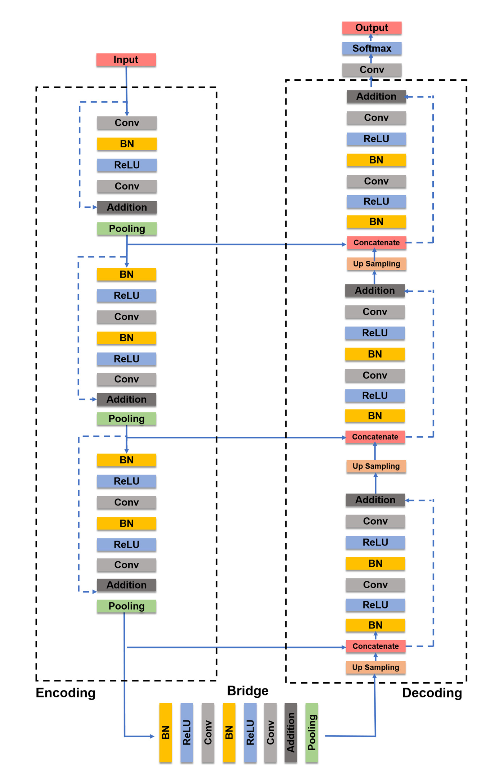
\includegraphics[width=0.6\textwidth]{./images/ResNet-architecture.png}
    \caption{Residual U-net model proposed by \cite{He2015} and used in \cite{Zheng2020}}
\end{figure}

The model was applied to a dataset composed by 450 OCT B-scans that were augmented to 1436 scans of 2048*1561 pixels. The performance was measured using the intraclass correlation coeficient (ICC) which is described as the level of resemblance between two or more samples of the belong to a common group defined by a particular set of characteristics. In Zheng's paper the groups were conformed by choroidal boundaries Bruch's Membrane and Choroidal Scleral Interface and a set of vasculature measurements such as the choroidal vascularity index (CVI), choroidal stromal index (CSI), luminal area (LA) ,stromal area (SA), the total choroidal area (TCA),and CT.

\begin{figure}[H]
    \centering
    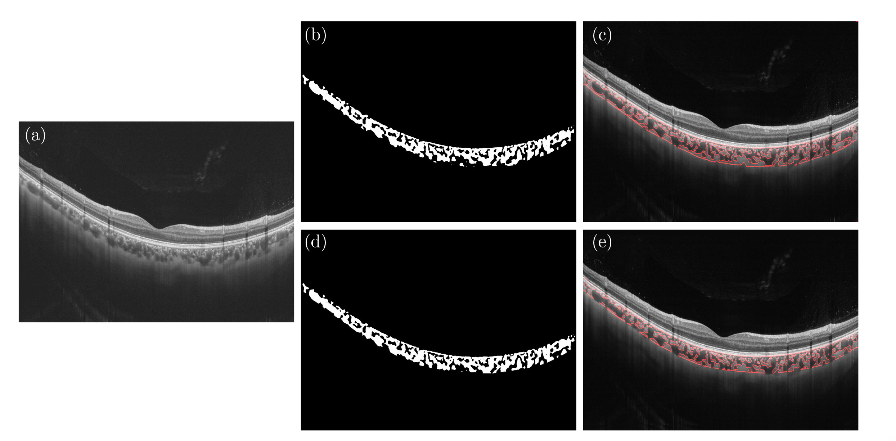
\includegraphics[width=0.8\textwidth]{./images/choroidal-segmentation-zheng.png}
    \caption{Predictions obtained by Zheng et al. (a) Raw OCT Scan (b) automatic identification of the upper and lower choroid boundaries; (c) binarization image of the choroid and (d) demarcation of luminal area (LA) and stromal area (SA) with red dotted line. \cite{Zheng2020}}
\end{figure}





\section{Discussion}\label{s:Discussion}

In this section we will detail the process of creating the framework from its inception point to evaluating the final output. In order to standardize its description we have chosen to fit our process to the Machine Learning workflow. 
\subsection{Data Collection}

Ronchetti could maybe explain us better what's the data collection process and the annotation process. We can say where the ophtalmologist come from, how many do we have. What is the collaboration with the hospital in hong kong, etc. OOOOR we can transfer the Data section in the introduction here.

\subsection{Data Preparation}\label{ss:datapreparation}

\subsubsection{Mask Segmentation}
\subsection{Model Development}
\subsection{Model Training}
\subsection{Model Evaluation}

\section{Results}\label{Results}


\newpage
\section{Conclusion}


\section{Future Work}

\markboth{}{}

\newpage

\bibliographystyle{plain} % We choose the "plain" reference style
\bibliography{bibli} % Entries are in the "bibi.bib" file




\newpage
\thispagestyle{empty}
\markboth{}{}
  \normalsize
\begin{center}
\huge{\textbf{ Declaration of Independence}}\\[40mm]
\end{center}
\large
We confirm that the above work has been produced by the authors without any unauthorized assistance and without the use of any other means than those indicated, and that I have marked as such all passages that have been taken literally or meaningfully from published or unpublished writings.\\[50mm]
Bienne, the \today

\newpage



\end{document}